%---------------------------------------------------------------
\chapter{Feedback Pollution}
%---------------------------------------------------------------

\begin{chapterabstract}
	\todoadd
\end{chapterabstract}

This chapter is based on the paper \cite{feedback-vmil}.

%---------------------------------------------------------------
\section{Motivation}
%---------------------------------------------------------------

Let's take the example in listing \ref{lst:pollution-motive} and consider disabled contextual dispatch in Ř and no OSR compilations of loops. The event log of the listing is demonstrated in \ref{fig:pollution-motive-baseline}.

\begin{listing}[H]
	\begin{minted}{R}
sum <- function(vec, init) {
  s <- init
  for (i in 1:length(vec))
    s <- s + vec[[i]]
  s
}

for (x in 1:1000) sum(doubles, 0.0)
for (x in 1:1000) sum(integers, 0L)
for (x in 1:1000) sum(doubles, 0.0)
  \end{minted}
	\caption{Motivating example for feedback pollution}\label{lst:pollution-motive}
\end{listing}

At first, we will execute the function \texttt{sum} with a vector of doubles. The type feedback will reflect that and after few executions, a compilation will get triggered, assuming on the types of arguments being double. This will speedup the execution significantly because the operations can be specialized for the double type.

Next when we run the function with integers, we fail the assumption on doubles, trigger a deoptimization and fallback to the baseline interpreted version. We also update the feedback information of \texttt{sum}, now reflecting both double and integer type. Because of this, the next function compilation cannot speculate on one specific type of an argument and instead uses a very general type (the only assumption made is that the value does not have any attributes). This makes the newly compiled native function about an order of a magnitude slower.

This is where we say that in the second compilation the \textit{type feedback slots are polluted}. They contain too general of an information; thus we specialize to a more general context and lose performance.

\begin{figure}
	\centering
	\begin{adjustwidth}{-3cm}{-3cm}
		\includediagram{5}
	\end{adjustwidth}
	\caption{Event log of listing \ref{lst:pollution-motive} without contextual dispatch}\label{fig:pollution-motive-baseline}
\end{figure}

If we consider contextual dispatch, the performance is better, but not ideal (illustrated in \ref{fig:pollution-motive-context}). Same as without the contextual dispatch, we first observe and speculate on the type double. The final version is compiled for a context of arguments being the double type \todo{reword}.

When we call with integers, we do not dispatch into the already compiled version, because the call context is disjunct with the context of the compiled version. Instead we run in the bytecode interpreter, updating the type feedback to also include integer. After few invocations, we compile for the second context and again we have to speculate on a more general type, resulting in a slower execution.

But contrary to the non-contextual dispatch, when we call \texttt{sum} with double type, it is dispatched again to the first compiled version, and thus its execution is as fast as the first time we called it.

\begin{figure}
	\centering
	\begin{adjustwidth}{-3cm}{-3cm}
		\includediagram{6}
	\end{adjustwidth}
	\caption{\todo{also update}Event log of listing \ref{lst:pollution-motive} with contextual dispatch}\label{fig:pollution-motive-context}
\end{figure}

%---------------------------------------------------------------
\section{Methodology}
%---------------------------------------------------------------

Our main goal is to quantify the pollution of the feedback vector. A pollution happens when between individual compilations the feedback vector changes, either because an interpreter has observed a new value or a native version fails on an assumption and deoptimizes. This implies that the first compilation cannot be polluted, hence we are interested in \textit{subsequent compilations} (or also \textit{recompilations}).

Formally, we define
\begin{itemize}
	\item{} \textit{polluted feedback slot} as a slot whose value at the point of compilation has changed from previous compilation,
	\item{} \textit{feedback pollution} as a ratio of the number of modified feedback slots to the total number of feedback slots,
	\item{} \textit{polluted compilation} as a compilation, where the feedback pollution is greater than 0,
	\item{} and \textit{function pollution} as a ratio between the polluted compilations and the total number of recompilations.
\end{itemize}

\todo{overview table}

Since the state of the feedback cannot go to a previous state (i.e. on an update, the feedback either stays the same or it is in a never before observed state), we can simply observe the state of the feedback slots when a compilation is triggered and compare it to the previous compilation.

For collecting the data, we used the recording tool introduced in the chapter \ref{ch:recording-tool}. As an input to the experiment, we used 16 benchmarks from the Ř benchmarks collection containing nearly 1300 lines of code and a Kaggle competition program, both outlined in chapter \ref{ch:1-corpus}. The Ř compiler is ran with default parameters, meaning that a function is compiled after 100 invocations. Compilations triggered by loop iterations are ignored.

%---------------------------------------------------------------
\section{Analysis}
%---------------------------------------------------------------

First, we will observe the the Kaggle code. Running the script, 315 functions are compiled and 146 of them are compiled more than once. A function compilation is triggered 970 times and out of these 824 are recompilations (2.6 recompilations on average per function). Overall, we have observed 90 polluted recompilations (10.9\%), where 19 recompilations have more than half of the slots polluted and 10 have all of the slots polluted.

Figure \ref{fig:kaggle-pollution} shows the function pollution in Kaggle. Each point represents a compilation, where the y-axis is showing an \textit{accumulated pollution}, i.e. the summed pollution of all subsequent compilations up to that point. On the x-axis, we show the functions that were compiled more than once.

\begin{figure}
	\centering
	\begin{adjustwidth}{-2cm}{-2cm}
		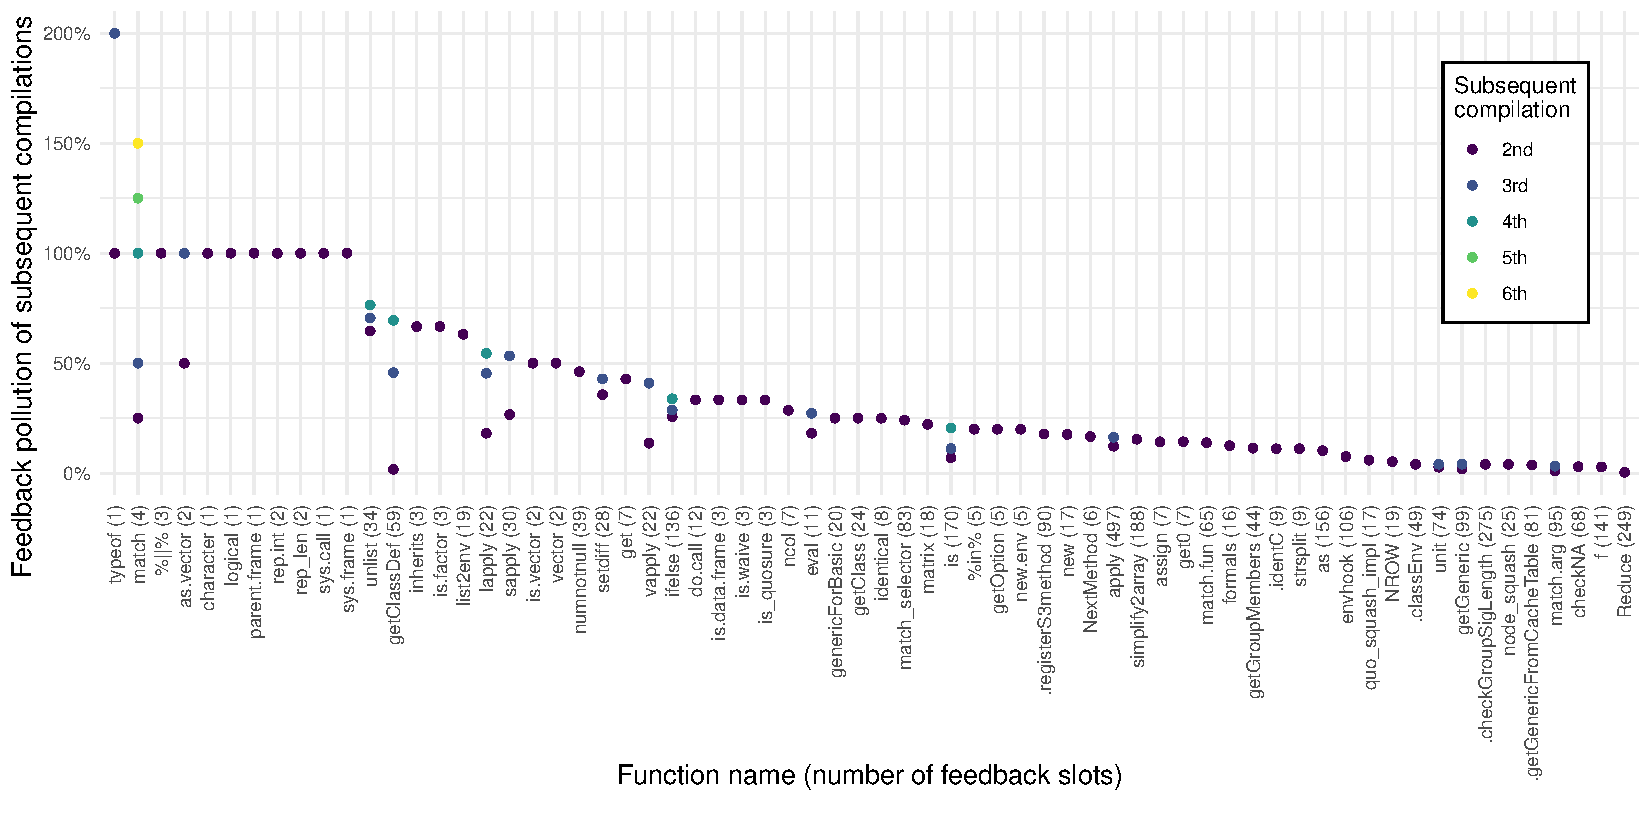
\includegraphics[width=1.3\textwidth]{figures/pollution/master/kaggle-function-pollution.pdf}
	\end{adjustwidth}
	\caption{Function pollution in Kaggle script, each point represents a compilation\cite{feedback-vmil}}\label{fig:kaggle-pollution}
\end{figure}

When we take as an example the function \texttt{typeof}, we have three compilations. The second compilation has a 100\% polluting and the third a 200\% pollution, meaning that both of the recompilations use all slots as polluted. The function is a wrapper around a C function that returns the type of the argument. It has a single parameter, to which the slot is connected to, and since it can be called with any type, it will always pollute when a new type is observed.

Looking at the benchmarks, we have observed much less compilations than in the Kaggle code. This is to be expected, as the benchmarks are mostly small numerical programs. In figure \ref{fig:bench-pollution} we can see the \textit{benchmark pollution}, which is the ratio of polluted recompilations out of all recompilations. Out of the 16 selected benchmarks, 10 of them have at least one polluted compilation. The overall ratio between polluted compilations is 8.2\%, which is very similar to the 10.9\% observed in the Kaggle code, but when looking at the function pollution, we have observed that out of 139 compiled functions there are 21 polluted functions (15.1\%). This is very likely due to the nature of the benchmarks, as they are numeric programs which are mostly using very few types. Still, a pollution can be observed and should be prevented.

\begin{figure}
	\centering
	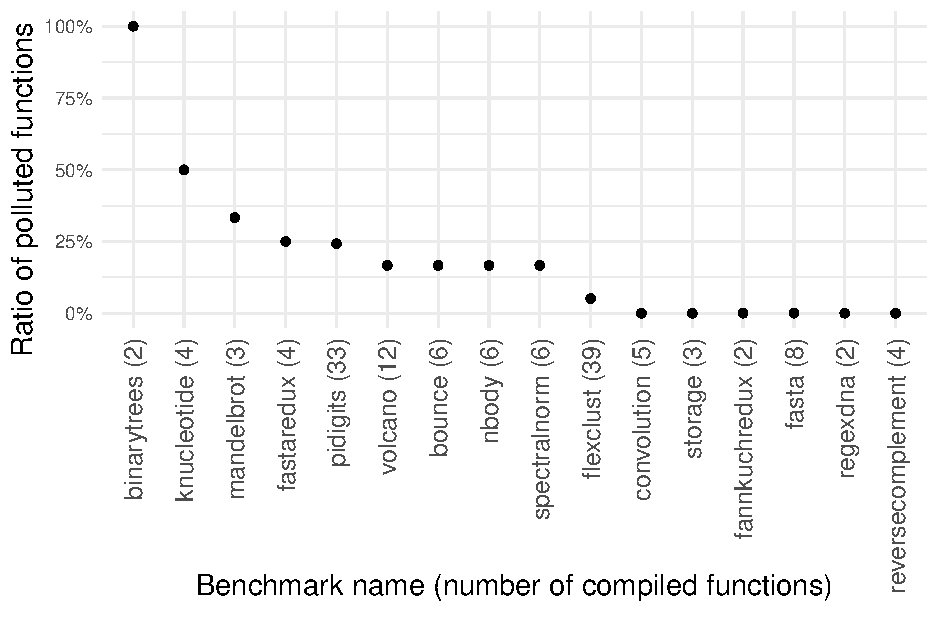
\includegraphics[width=0.7\textwidth]{figures/pollution/master/benchmark-pollutionBW.pdf}
	\caption{Pollution of functions in benchmarks\cite{feedback-vmil}}\label{fig:bench-pollution}
\end{figure}

Splitting the pollution by a feedback slot type, the observed values are taking most of the pollution. Out of the 11,199 slots in the Kaggle code, 0.5\% of observed calls, 2.7\% of observed tests, and 5.7\% of observed values are polluted. This is not surprising, as the type feedback slots are the slots with most variability.

\todo{the polymorphic functions}

%---------------------------------------------------------------
\subsubsection*{Summary}
%---------------------------------------------------------------

In table \ref{tbl:pollution-summary} is a summary of the feedback compilation in the benchmarks and in the Kaggle code. We can see that feedback pollution happens in both the Kaggle code as well as in the benchmarks, although the benchmarks have a lower pollution rates, mostl likely due to the stable nature of the code.

We have observed that pollution is most likely caused by polymorphic functions that are called often with different types, but other causes for pollution can be a global state.

Most of the polluted slots are the observed values.

\begin{table}[H]
	\centering
	\begin{tabular}{llll}
		\hline
		                      & Kaggle      & Benchmarks  \\
		\hline
		Lines of code         & 108         & 1268        \\
		Compilations          & 970         & 257         \\
		Polluted compilations & 90 (10.9\%) & 21 (8.2\%)  \\
		Compiled functions    & 315         & 139         \\
		Polluted functions    & 66 (21\%)   & 21 (15.1\%) \\
		\hline
	\end{tabular}
  \caption{Summary of the feedback pollution in the corpus\cite{feedback-vmil}}\label{tbl:pollution-summary}
\end{table}


The code of the analysis is freely available at GitLab\footnote{\url{https://gitlab.com/rirvm/splitfeedback-experiments/-/tree/artifact}} as part of the VMIL paper\cite{feedback-vmil} aritfact.

%---------------------------------------------------------------
\section{Pollution Prevention}
%---------------------------------------------------------------

After observing that a feedback pollution is a real phenomenon, we propose a way to reduce it.

One way to reduce the pollution is to split the feedback vector into multiple different ones. Since Ř already employs a contextual dispatch, the constructed dispatch could be reused by the feedback, constructing a unique vector for each call context the function is invoked with. A split feedback was implemented by Michal Štěpánek as a part of his master thesis\cite{michal2025obohaceny}. However, this solution brought new problems, as now the observed information is much sparser and needs to be merged from multiple vectors. Splitting the feedback also negativaly impacts the interpreter performance, and complicates function compilation.

Another approach would be to implement a \textit{feedback decay}. The idea is that the feedback information in every slot would slowly \textit{decay} as new information is observed. This will need to be finely tuned, as very quickly the JIT could be stuck in a \textit{deopt loop}, compiling a function just to trigger a deoptimization next time it is invoked.
